\documentclass{standalone}
\usepackage{tikz}
\begin{document}
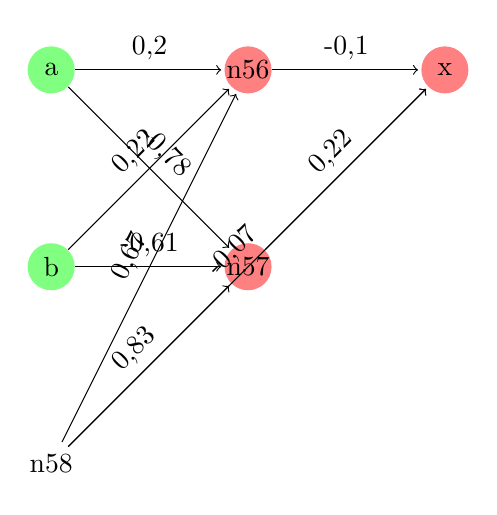
\begin{tikzpicture}[shorten >=1pt,->,draw=black!,node distance=2.5cm]
\tikzstyle{neuron}=[circle,fill=black!25,minimum size=17pt,inner sep=0pt]
\tikzstyle{constant}=[neuron, fill=white!50];
\tikzstyle{identity}=[neuron, fill=green!50];
\tikzstyle{sigmoid}=[neuron, fill=red!50];
\node [identity] (a) {a};
\node [identity,below of=a] (b) {b};
\node [constant,below of=b] (n58) {n58};
\node [sigmoid,right of=a] (n56) {n56};
\node [sigmoid,below of=n56] (n57) {n57};
\node [sigmoid,right of=n56] (x) {x};
\path[every node/.style={sloped,anchor=south,auto=false}]
(a) edge node {0,2} (n56)
(a) edge node {-0,78} (n57)
(b) edge node {-0,61} (n57)
(b) edge node {0,22} (n56)
(n58) edge node {-0,07} (x)
(n58) edge node {0,83} (n57)
(n58) edge node {0,67} (n56)
(n56) edge node {-0,1} (x)
(n57) edge node {0,22} (x)
;\end{tikzpicture}
\end{document}